\newcommand{\Depth}{2}
\newcommand{\Height}{2}
\newcommand{\Width}{2}

\newcommand{\ncube}[3]{
\coordinate (O) at (#1);
\coordinate (A) at (0,-#2,0);
\coordinate (B) at (0,-#2,-#2);
\coordinate (C) at (0,0,-#2);
\coordinate (D) at (#2,0,0);
\coordinate (E) at (#2,-#2,0);
\coordinate (F) at (#2,-#2,-#2);
\coordinate (G) at (#2,0,-#2);

\draw[blue,fill=yellow!30,opacity=#3] (O) -- (C.center) -- (G) -- (D) -- cycle;% Bottom Face
\draw[blue,fill=blue!30,opacity=#3] (O) -- (A) -- (E) -- (D) -- cycle;% Back Face
\draw[blue,fill=red!10,opacity=#3] (O) -- (A) -- (B) -- (C) -- cycle;% Left Face
\draw[blue,fill=red!20,opacity=#3] (D) -- (E) -- (F) -- (G) -- cycle;% Right Face
\draw[blue,fill=red!20,opacity=#3] (C) -- (B) -- (F) -- (G) -- cycle;% Front Face
\draw[blue,fill=red!20,opacity=#3] (A) -- (B) -- (F) -- (E) -- cycle;% Top Face}
}

\newcommand{\ccube}[5]{
\coordinate (O) at (#1);
\coordinate (A) at (0,-#2,0);
\coordinate (B) at (0,-#2,-#3);
\coordinate (C) at (0,0,-#3);
\coordinate (D) at (#4,0,0);
\coordinate (E) at (#4,-#2,0);
\coordinate (F) at (#4,-#2,-#3);
\coordinate (G) at (#4,0,-#3);

\draw[blue,fill=yellow!30,opacity=#5] (O) -- (C.center) -- (G) -- (D) -- cycle;% Bottom Face
\draw[blue,fill=blue!30,opacity=#5] (O) -- (A) -- (E) -- (D) -- cycle;% Back Face
\draw[blue,fill=red!10,opacity=#5] (O) -- (A) -- (B) -- (C) -- cycle;% Left Face
\draw[blue,fill=red!20,opacity=#5] (D) -- (E) -- (F) -- (G) -- cycle;% Right Face
\draw[blue,fill=red!20,opacity=#5] (C) -- (B) -- (F) -- (G) -- cycle;% Front Face
\draw[blue,fill=red!20,opacity=#5] (A) -- (B) -- (F) -- (E) -- cycle;% Top Face}
}

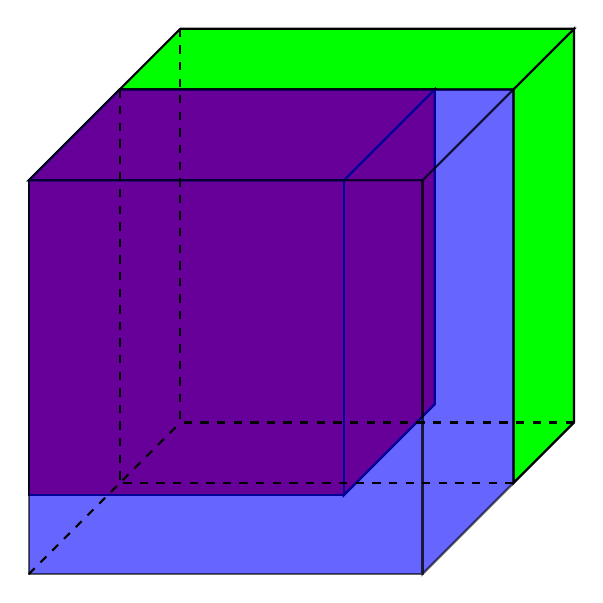
\begin{tikzpicture}[
		cube/.style={thick},
		cube hidden/.style={thick,dashed}]

  % origin
  \coordinate (o) at (0,0,0);

  % coordinates of the front of the low rank part
  \coordinate (a) at (5,0,0);
  \coordinate (b) at (0,5,0);
  \coordinate (c) at (5,5,0);

  % coordinates of the back of the low rank part
  \coordinate (d) at (0,0,-3);
  \coordinate (e) at (5,0,-3);
  \coordinate (f) at (0,5,-3);
  \coordinate (g) at (5,5,-3);

  % coordinates of the front of the kernel part
  \coordinate (h) at (0,1,0);
  \coordinate (i) at (4,1,0);
  \coordinate (j) at (4,5,0);

  \coordinate (k) at (0,1,-3);
  \coordinate (l) at (4,1,-3);
  \coordinate (m) at (4,5,-3);

  \coordinate (n) at (0,0,-5);
  \coordinate (p) at (5,0,-5);
  \coordinate (q) at (0,5,-5);
  \coordinate (r) at (5,5,-5);


  % high rank matrices part
  \draw[cube,fill=green] (g) -- (r) -- (p) -- (e) -- cycle;
  \draw[cube,fill=green] (g) -- (r) -- (q) -- (f) -- cycle;


  % kernel part
  \draw[cube,fill=red,] (j) -- (m) -- (l) -- (i) -- cycle;% Right Face
  \draw[cube,fill=red] (b) -- (h) -- (i) -- (j) -- cycle;% Front Face
  \draw[cube,fill=red] (b) -- (f) -- (m) -- (j) -- cycle;% Top Face

  % low rank matrices part
  \draw[cube,fill=blue,opacity=0.6] (a) -- (e) -- (g) -- (c) -- cycle;% Right Face
  \draw[cube,fill=blue,opacity=0.6] (o) -- (a) -- (c) -- (b) -- cycle;% Front Face
  \draw[cube,fill=blue,opacity=0.6] (b) -- (c) -- (g) -- (f) -- cycle;% Top Face


  \draw[cube hidden] (o) -- (n);
  \draw[cube hidden] (q) -- (n);
  \draw[cube hidden] (p) -- (n);

  \draw[cube hidden] (e) -- (d);
  \draw[cube hidden] (f) -- (d);


  % \draw[cube hidden,fill=red!30] (o) -- (d) -- (e) -- (a) -- cycle;% Bottom Face
  %\draw[cube hidden,fill=red!30] (d) -- (e) -- (g) -- (f) -- cycle;% Back Face
  %\draw[cube hidden,fill=red!30] (o) -- (d) -- (f) -- (b) -- cycle;% Left Face



  % drawing the kernel part
  %\draw[black,fill=red!30,opacity=0.8] (o) -- (c.center) -- (g) -- (d) -- cycle;% Bottom Face
  %\draw[black,fill=red!30,opacity=0.8] (o) -- (a) -- (e) -- (d) -- cycle;% Back Face
  %\draw[black,fill=red!30,opacity=0.8] (o) -- (a) -- (b) -- (c) -- cycle;% Left Face
  %\draw[black,fill=red!30,opacity=0.8] (d) -- (e) -- (f) -- (g) -- cycle;% Right Face
  %\draw[black,fill=red!30,opacity=0.8] (c) -- (b) -- (f) -- (g) -- cycle;% Front Face
  %\draw[black,fill=red!30,opacity=0.8] (a) -- (b) -- (f) -- (e) -- cycle;% Top Face

%\ccube{O}{5}{5}{5}{0.2}
%\ncube{o}{4}{0.8}
%\ccube{o}{5}{4}{5}{0.2}

%\coordinate (Oa) at (0,0,-4);
%\coordinate (Aa) at (0,-5,-4);
%\coordinate (Ba) at (0,-5,-5);
%\coordinate (Ca) at (0,0,-5);
%\coordinate (Da) at (5,0,-4);
%\coordinate (Ea) at (5,-5,-4);
%\coordinate (Fa) at (5,-5,-5);
%\coordinate (Ga) at (5,0,-5);

%\draw[blue,fill=yellow!30,opacity=0.5] (Oa) -- (Ca.center) -- (Ga) -- (Da) -- cycle;% Bottom Face
%\draw[blue,fill=blue!30,opacity=0.5,densely dashed] (Oa) -- (Aa) -- (Ea) -- (Da) -- cycle;% Back Face
%\draw[blue,fill=red!10,opacity=0.5] (Oa) -- (Aa) -- (Ba) -- (Ca) -- cycle;% Left Face
%\draw[blue,fill=red!20,opacity=0.5] (Da) -- (Ea) -- (Fa) -- (Ga) -- cycle;% Right Face
%\draw[blue,fill=red!20,opacity=0.5] (Ca) -- (Ba) -- (Fa) -- (Ga) -- cycle;% Front Face
%\draw[blue,fill=red!20,opacity=0.5] (Aa) -- (Ba) -- (Fa) -- (Ea) -- cycle;% Top Face}

%\draw ($(C) +(0,-0.5)$) -- node[below,sloped]{label 1} ($(O)+(0,-0.5)$);
%\draw ($(C) +(0,-0.5)$) -- node[below,sloped]{label 2} ($(G)+(0,-0.5)$);
%\draw ($(A) +(0.5,0)$) -- node[sloped,above]{label 3} ($(O)+(0.5,0)$);

%% Following is for debugging purposes so you can see where the points are
%% These are last so that they show up on top
%\foreach \xy in {o, a, b, c, d, e, f, g, h, i, j, k, l, m,p,q,r}{
%    \node at (\xy) {\xy};
%}
\end{tikzpicture}
